\documentclass[10pt,pdf,hyperref={unicode}]{beamer}

\usepackage{graphicx}
\graphicspath{{./figs/}}

\mode<presentation> {
	\usetheme{Warsaw}
%	\usetheme{chpc}
	  
	\setbeamercovered{transparent}
  % or whatever (possibly just delete it)
}

\usepackage[english]{babel}
%\usepackage[utf8x]{inputenc}

%\usepackage{amsmath}
\usepackage{bm}
\usepackage{tikz}
\usepackage{pgfplots}

\title[] % (optional, use only with long paper titles)
{Algorithm of Time Step Selection for Numerical Solution of Boundary Value Problem for Parabolic  Equations}

%\subtitle
%{Include Only If Paper Has a Subtitle}

\author[] % (optional, use only with lots of authors)
{Petr Vabishchevich \inst{1,2} \and \underline{Aleksandr Vasilev \inst{2}}}
% - Give the names in the same order as the appear in the paper.
% - Use the \inst{?} command only if the authors have different
%   affiliation.

\institute[Universities of Somewhere and Elsewhere] % (optional, but mostly needed)
{
\inst{1}  Nuclear Safety Institute, Russian Academy of Sciences, Moscow, Russia
\\
\vspace{1mm}
\inst{2} North-Eastern Federal University, Yakutsk, Russia
}

% - Use the \inst command only if there are several affiliations.
% - Keep it simple, no one is interested in your street address.

\date[June  20-25, 2018] % (optional, should be abbreviation of conference name)
{AMiTaNS, June 20-25, 2018 Albena}
% - Either use conference name or its abbreviation.
% - Not really informative to the audience, more for people (including
%   yourself) who are reading the slides online

\subject{Theoretical Computer Science}
% This is only inserted into the PDF information catalog. Can be left
% out. 

% ����� � ���������
\graphicspath{{./figs/}}
\newcommand{\grad}{\mathop{\rm grad}\nolimits}
\renewcommand{\div}{\mathop{\rm div}\nolimits}
\newcommand{\const}{\mathop{\rm const}\nolimits}

\begin{document}

\begin{frame}
  \titlepage
\end{frame}

%{
%  \begin{frame}<beamer>
%    \tableofcontents
%  \end{frame}
%}

\section{Introduction}
\begin{frame}{Introduction}
\begin{small}
The problem of the time step control is relatively well developed for the Cauchy problem solution of differential equations systems. (Gear 1971, Hairer Norsett Wanner 1987, Asher 1998, ...)
The basic approach is to use additional calculations at a new time step to estimate the approximate solution. The time step is estimated using the theoretical asymptotic dependence of the accuracy on time step.
\vspace{1mm}

\visible<2,3>{
Additional calculations for estimating the error of the approximate solution can be carried out in different ways. The best-known strategy is connected with the solution of the problem on a separate time interval using the given step (the first solution) and with a step two times smaller (the second solution). The noted ways of selecting the time step are related to the class of a posteriori accuracy estimation methods.
The decision as to suitable the time step or the re-calculation is accepted only after the calculation is completed.
}

\visible<3>{
\vspace{1mm}
In this paper we consider in fact a priori choice of the time step in the approximate solution of boundary value problems for parabolic equations. The proposed algorithm allows a gain in CPU time with respect to the fine mesh calculation at the same calculation accuracy.
}
\end{small}
\end{frame}

\section{Problem description}
\subsection{Parabolic equation}
\begin{frame}{Problem description}
Consider second-order parabolic equation
\[
   \frac{\partial u}{\partial t} 
   - \sum_{\alpha =1}^{m}
   \frac{\partial }{\partial x_\alpha} 
   \left ( k({\bm x},t)  \frac{\partial u}{\partial x_\alpha} \right ) + s({\bm x},t) u = f({\bm x},t),
   \quad {\bm x}\in \Omega,
   \quad 0 < t \leq  T,
\]
where
$\underline{k} \leq k({\bm x}) \leq  \overline{k}, \ {\bm x} \in \Omega, \ \underline{k} > 0$.
\vfill

%\visible<2>{
Boundary condition
\[
   u({\bm x},t) = g({\bm x},t),
   \quad {\bm x}\in \partial \Omega,
   \quad 0 < t \leq  T.
\]

Initial condition
\[
   u({\bm x},0) = u^0({\bm x}),
   \quad {\bm x}\in \Omega.
\]
%}
\end{frame}

\subsection{Operator notation}
\begin{frame}{Operator notation}
Cauchy problem for linear equation
\[
  \frac{du}{dt} + A(t) u = f(t),
  \quad 0 < t \leq T,
\]
with following initial condition
\[
   u(0) = u_0.
\]
The problem is considered in a finite-dimensional Hilbert space $H$. 
\vfill

\visible<2>{
Assume $A(t) \geq 0$ in $H$ then, for the Cauchy problem we have a stability estimate with respect to the initial data and the right-hand side
\[
  \|u(t)\| \leq \|u_0\| + \int_{0}^{t} \|f(\theta) \| d \theta .
\]
}
\end{frame}

\subsection{Solution evaluation}
\begin{frame}{Solution evaluation}
Introduce irregular time grid
\[
 t^0=0, \quad t^{n+1} = t^n + \tau^{n+1},
 \quad n = 0,1, ..., N-1,
 \quad t^n = T .   
\] 
For an approximate solution the implicit scheme are used
\[
  \frac{y^{n+1} - y^{n}}{\tau^{n+1}} + A^{n+1} y^{n+1} = f^{n+1},
  \quad n = 0,1, ..., N-1,
\]
and initial condition $y^0 = u^0.$

\vfill

\visible<2>{
For an approximate solution under restriction  $A^{n+1} \geq 0$:

Layerwise estimate
\[
 \|y^{n+1}\| \leq \|y^{n}\| + \tau^{n+1} \|f^{n+1}\|.
\]

Difference estimate
\[
 \|y^{n+1}\| \leq \|u^{0}\| + \sum_{k=0}^{n} \tau^{k+1} \|f^{k+1}\|.
\]
}
\end{frame}

\subsection{Solution error}
\begin{frame}{Solution error}
For the error of the approximate solution $z^n = y^n - u^n$:
\[
  \frac{z^{n+1} - z^{n}}{\tau^{n+1}} + A^{n+1} z^{n+1} = \psi^{n+1},
  \quad n = 0,1, ..., N-1,  
\] 
\[
 z^0 = 0.
\] 

Where the approximation error is
\[
 \psi^{n+1} = f^{n+1} -
 \frac{u^{n+1} - u^{n}}{\tau^{n+1}} - A^{n+1} u^{n+1} . 
\]

\visible<2>{
Similarly, we have an difference estimate for the error
\[
  \|z^{n+1}\| \leq \sum_{k=0}^{n} \tau^{k+1} \|\psi^{k+1}\| .
\]

Then we obtain
\[
 \|z^{n+1}\| \leq \delta t^{n+1}.
\] 
}
\end{frame}

\section{Time step estimate}
\subsection{Algorithm}
\begin{frame}{Time step selection algorithm}
\begin{enumerate}
\item 
Predictable time step: $\widetilde{\tau}^{n+1} = \gamma \tau^n$ (eg $\gamma=1.25$ or $1.5$)
\vspace{2mm}

\visible<2,3,4,5>{
\item Predictive solution $\widetilde{y}^{n+1}$: an explicit scheme, $\widetilde{t}^{n+1} = t^n + \widetilde{\tau}^{n+1}$
}
\vspace{2mm}

\visible<3,4,5>{
\item Estimation of approximation error: by found $\widetilde{y}^{n+1}$ from an implicit scheme
}
\vspace{2mm}

\visible<4,5>{
\item Step selection $\tau^{n+1}$: $\ \|\psi^{n+1}\| \approx \delta$
}
\vspace{2mm}

\visible<5>{
\item Solution on a new time layer $y^{n+1}$: an implicit scheme, $t^{n+1}=t^n + \tau^{n+1}$
}
\end{enumerate}
\end{frame}

\subsection{Calculated formulas}
\begin{frame}{Calculated formulas}
The predictive solution $\widetilde{y}^{n+1} $  is defined from
\[
  \frac{\widetilde{y}^{n+1} - y^{n}}{\widetilde{\tau}^{n+1}} + A^{n} y^{n} 
  = f^{n} .
\]
The approximation error of predictive solution
\[
 \widetilde{\psi}^{n+1}  = \widetilde{f}^{n+1} -
 \frac{\widetilde{y}^{n+1} - y^{n}}{\widetilde{\tau}^{n+1}} -
 \widetilde{A}^{n+1} \widetilde{y}^{n+1} . 
\]
\visible<2>{
We match error $\widetilde{\psi}^{n+1}$  with step $\widetilde{\tau}^{n+1}$, and $\psi^{n+1}$ with step $\tau^{n+1}$:
\[
  \bar{\tau}^{n+1} = \gamma_{n+1} \tau^n,
  \quad \gamma_{n+1} = \frac{\delta}{\|\widetilde{\psi}^{n+1}\|}  \gamma .
\]
}
\end{frame}

\begin{frame}{Calculated formulas continued}
The needed time step
\[
 \tau^{n+1} \leq \bar{\tau}^{n+1},
 \quad  \tau^{n+1} \leq \widetilde{\tau}^{n+1},
 \quad
  \tau^{n+1} = \max \big \{\tau^0, \min \{\gamma_{n+1}, \gamma \} \tau^n \big \}. 
\] 

The approximation error has the first order in time
\[
\widetilde{\psi}^{n+1} = \mathcal{O} (\widetilde{\tau}_{n+1}).
\]

\visible<2>{
In view of this, we set 
\[
 \|\widetilde{\psi}^{n+1} \| \leq \|\widetilde{f}^{n+1} - f^n  -
 (\widetilde{A}^{n+1} - A^n) y^n -
 \widetilde{A}^{n+1} (\widetilde{y}^{n+1} - y^n) \| .
\]

Calculated formula for time step
\[
  \gamma_{n+1} = \frac{\delta}{ \|\widetilde{f}^{n+1} - f^n  -
  (\widetilde{A}^{n+1} - A^n) y^n  -
  \widetilde{A}^{n+1} (\widetilde{y}^{n+1} - y^n) \| } \gamma .
\]
}
\end{frame}

\section{Test problem}
\subsection{General description}
\begin{frame}{Model}
Consider the boundary problem for a 1D parabolic equation
\[
  \frac{\partial u}{\partial t} - \frac{\partial^2 u}{\partial x^2} + p(t) u = f(t),
  \quad 0 < x < 1,
  \quad 0 < t \leq  T ,  
\]
with boundary and initial conditions
\[
  u(0, t) = 0,
  \quad u(1,t) = 0,
  \quad 0 < t \leq  T ,    
\]
\[
  u(x,0) = u^0(x),
  \quad  \quad 0 <  x <  1 .
\]

\visible<2>{
The operator $A(t)$  is given in the form 
\[
 A u = - \frac{1}{h^2} (u(x+h) - 2 u(x) + u(x-h)) + p(t) u(x),
 \quad x \in \omega . 
\] 
The operator $A(t)$ is selfadjoint and for $p(t) \geq 0$ is positive definite in $H$.
Thus, after space approximating, we arrive at the original problem.
}
\end{frame}


\begin{frame}{Problem}
The problem is considered for $T = 0.1,\ \tau^0=10^{-6}$  with a discontinuous coefficient $p(t)$ and discontinuous right-hand side $f(t)$:
\[
  p(t) = \left \{
  \begin{split}
  \lambda  t, & \quad 0 < t \leq 0.075, \\
  0, & \quad 0.075 < t \leq 0.1 , \\   
  \end{split}  
  \right . 
\]  
\[
  f(t) = \left \{
  \begin{split}
  0, & \quad 0 < t \leq 0.05, \\
  \chi  e^{-10 (t-0.05)}, & \quad 0.05 < t \leq 0.1 . \\   
  \end{split}  
  \right . 
\]

\visible<2>{
We consider the case when the initial condition is taken in the form:
\[
  u^0(x) = \sin^\sigma (\pi x),
  \quad  \quad 0 <  x <  1 .
\] 
For the basic variant, we set
\[
 \lambda = 100,
 \quad \chi = 10, 
 \quad \sigma = 0.5 . 
\] 
}
\end{frame}

\begin{frame}{Comparing}
The accuracy of the approximate solution was estimated from the reference solution, that a numerical solution on a fine grid in time ($\tau=1 \cdot 10^{-7} $).\\
\vspace{1em}
The error is estimated in the norm of $ L_2 (\omega)$ ($\varepsilon_2 = \| \cdot \|$) or $L_\infty (\omega)$ ($\varepsilon_\infty=\| \cdot \|_\infty$), where
\[
  \| u \|_\infty = \max_ {x \in \omega} |u (x)|.
\]
\end{frame}

\subsection{Computational results}
\begin{frame}{Uniform grid}
\begin{center}
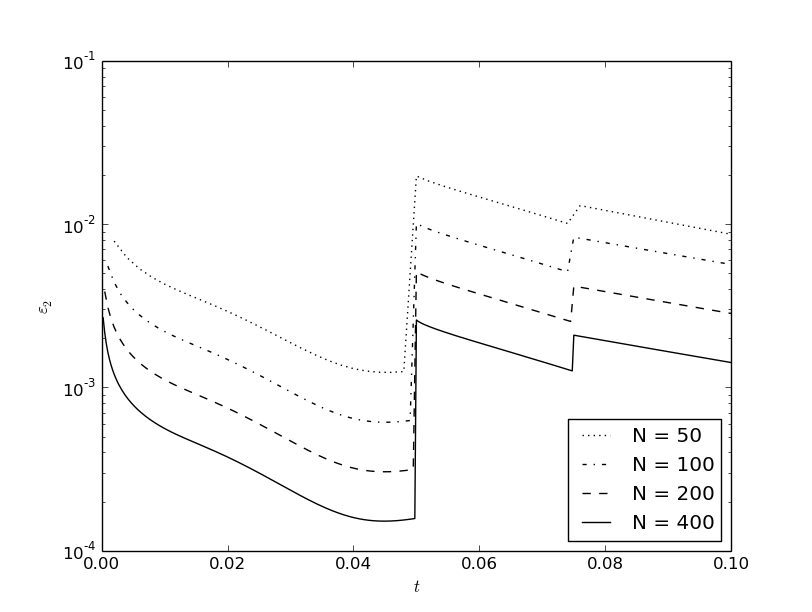
\includegraphics[width=0.8\linewidth] {ts_model/1.png}\\
Error in $L_2(\omega)$.
\end{center}
\end{frame}

\begin{frame}{Uniform grid}
\begin{center}
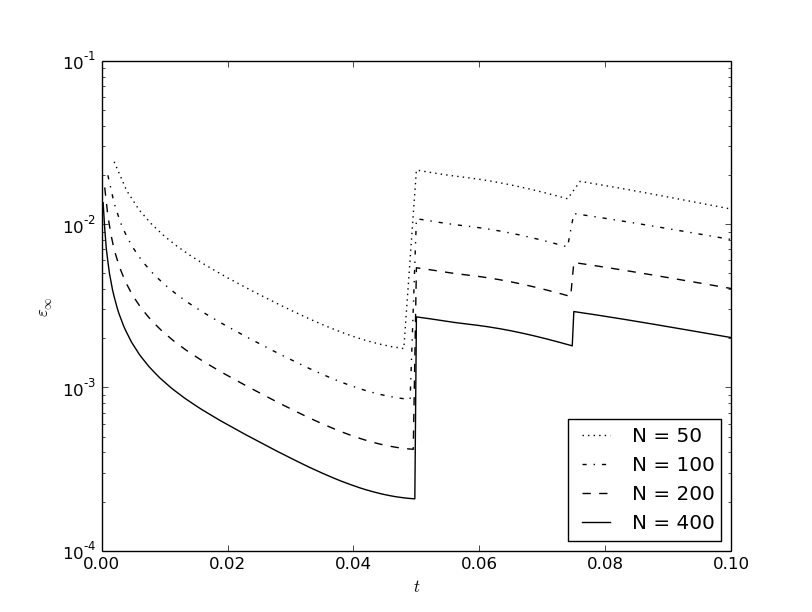
\includegraphics[width=0.8\linewidth] {ts_model/2.png}\\
Error in $L_\infty (\omega)$.
\end{center}
\end{frame}

\begin{frame}{Irregular grid}
\begin{center}
  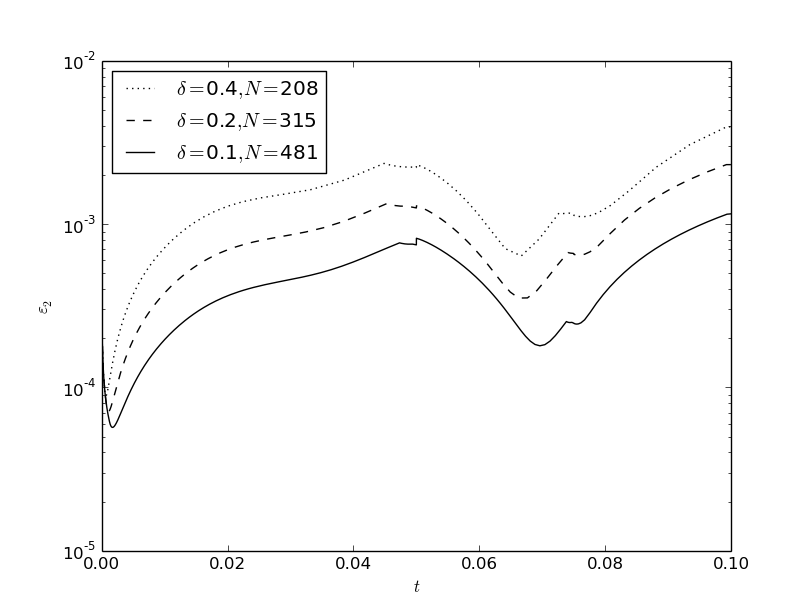
\includegraphics[width=0.8\linewidth] {ts_model/4.png}\\
  Error in $L_2(\omega)$. 
\end{center}
\end{frame}

\begin{frame}{Irregular grid}
\begin{center}
    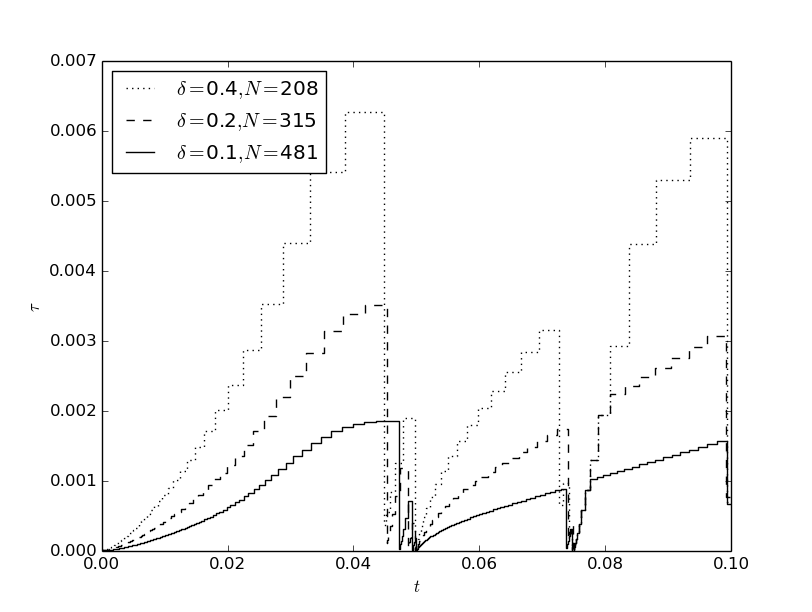
\includegraphics[width=0.8\linewidth] {ts_model/3.png} \\
    Time steps.
\end{center}
\end{frame}

\begin{frame}{Three layered scheme}
We can also use more accurate difference schemes to find the predictive solution.
The results of calculations using a three-layer explicit scheme.
\\
\begin{center}
 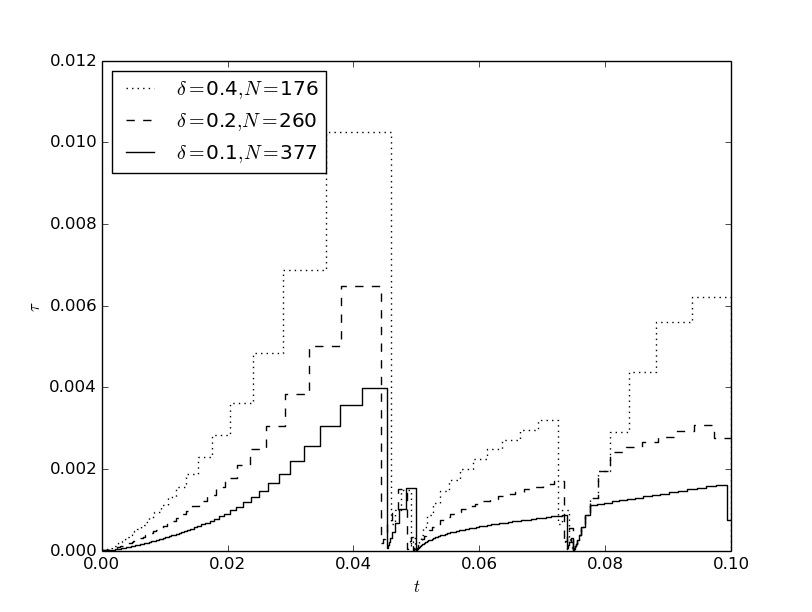
\includegraphics[width=0.7\linewidth] {ts_model/7.png}\\
Time steps.
\end{center}
\end{frame}

\begin{frame}{Three layered scheme}
\begin{center}
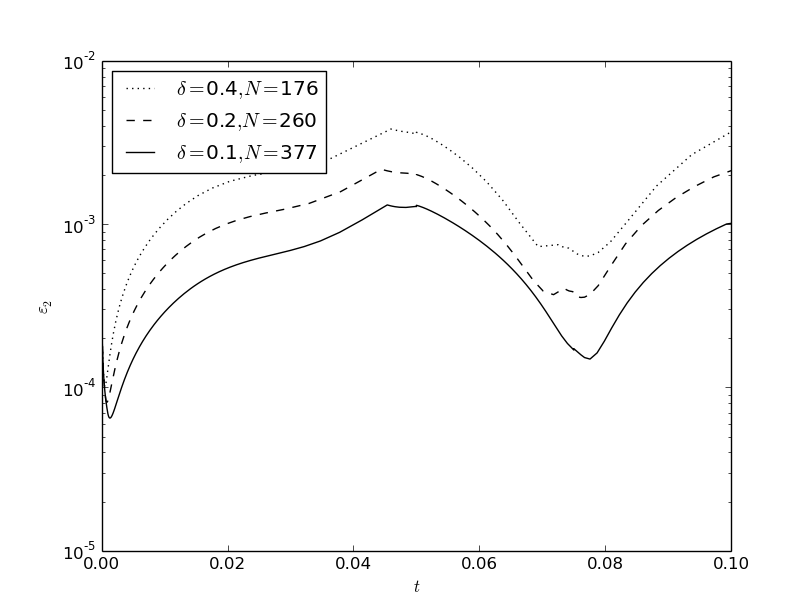
\includegraphics[width=0.8\linewidth] {ts_model/8.png}\\
Error on irregular grid.
\end{center}
\end{frame}

\begin{frame}{Gamma}
  \begin{center}
    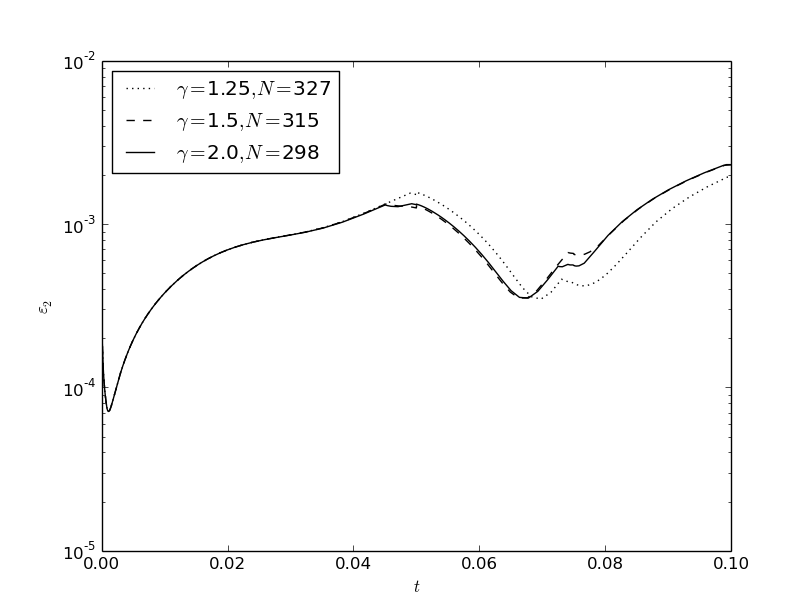
\includegraphics[width=0.8\linewidth] {ts_model/10.png}\\
  Error in $L_2(\omega)$. 
\end{center}
\end{frame}

\begin{frame}{Gamma}
 The effect of increase of the time step parameter is insignificant.\\
\begin{center}
    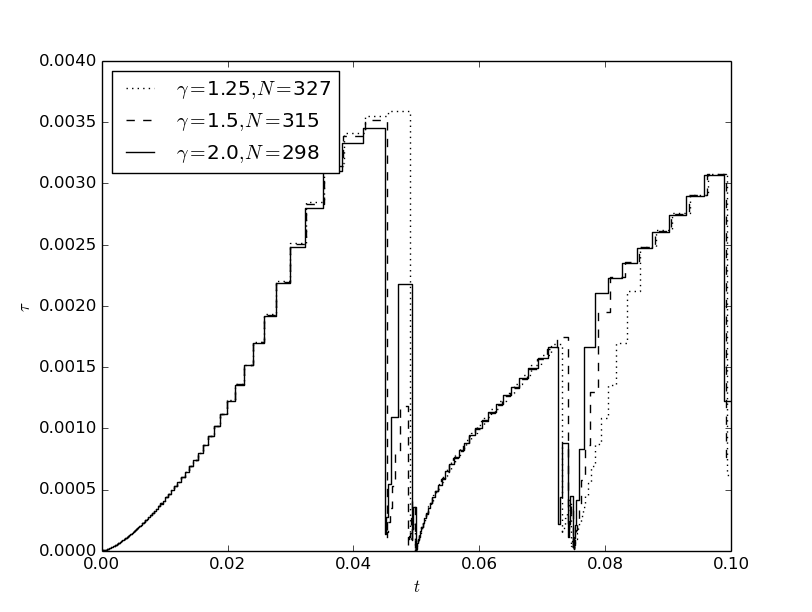
\includegraphics[width=0.8\linewidth] {ts_model/9.png}\\
	Time steps.
\end{center}
\end{frame}


\begin{frame}{Initial condition parameter}
\begin{center}
    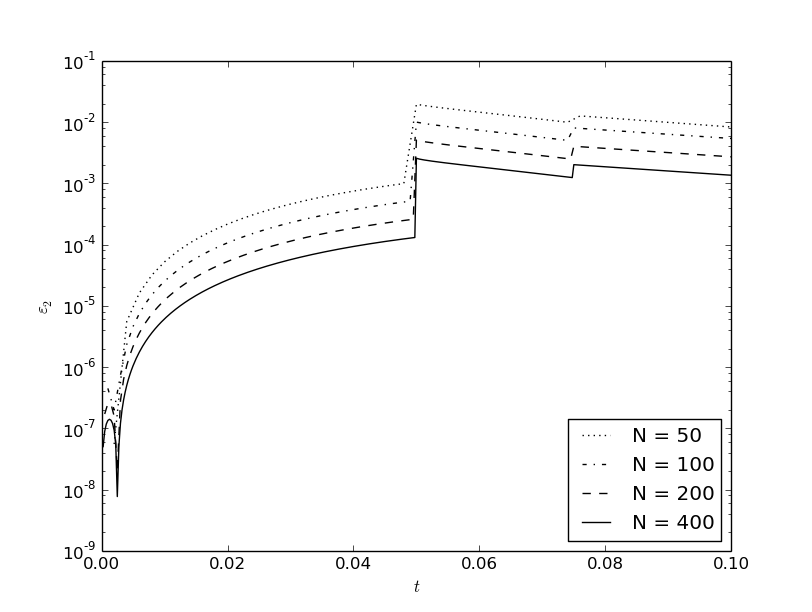
\includegraphics[width=0.8\linewidth] {ts_model/11.png}\\
	Error on uniform grid at $\sigma = 1$
\end{center}
\end{frame}

\begin{frame}{Initial condition parameter}
\begin{center}
    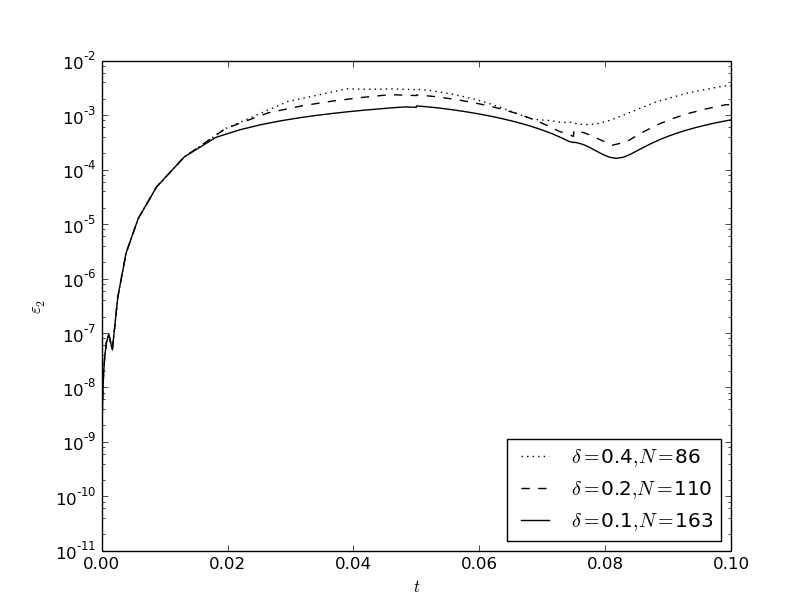
\includegraphics[width=0.8\linewidth] {ts_model/13.png}\\
	Error on irregular grid at $\sigma = 1$
\end{center}
\end{frame}

\begin{frame}{Initial condition parameter}
\begin{center}
Other parameters do not affect.\\
    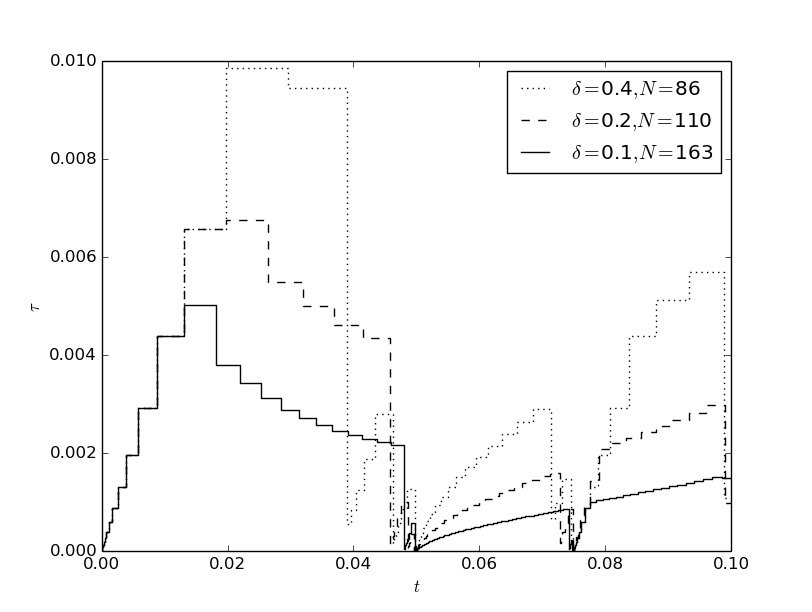
\includegraphics[width=0.8\linewidth] {ts_model/12.png}\\
	Time steps at $\sigma = 1$
\end{center}
\end{frame}

\begin{frame}{Crank-Nicolson scheme}
\begin{center}
   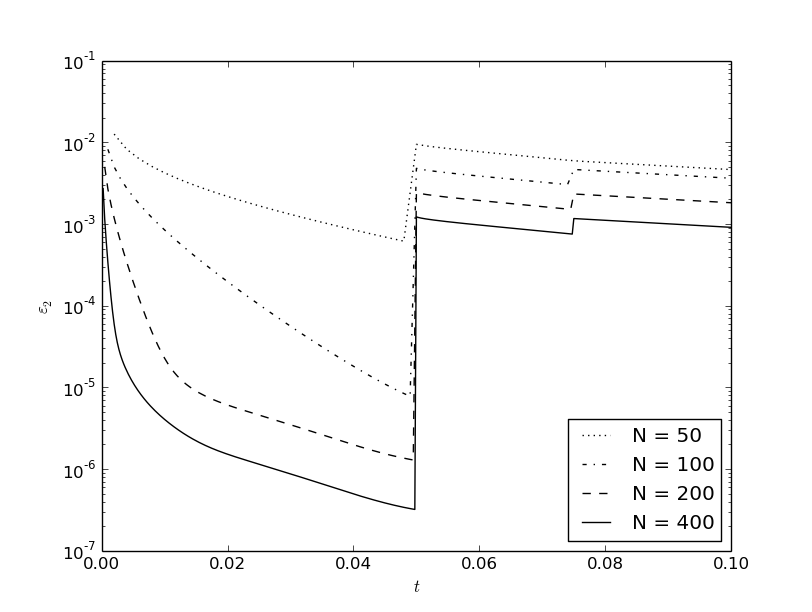
\includegraphics[width=0.8\linewidth] {ts_model/14.png}\\
	Error on uniform grid.
\end{center}
\end{frame}

\begin{frame}{Crank-Nicolson scheme}
\begin{center}
   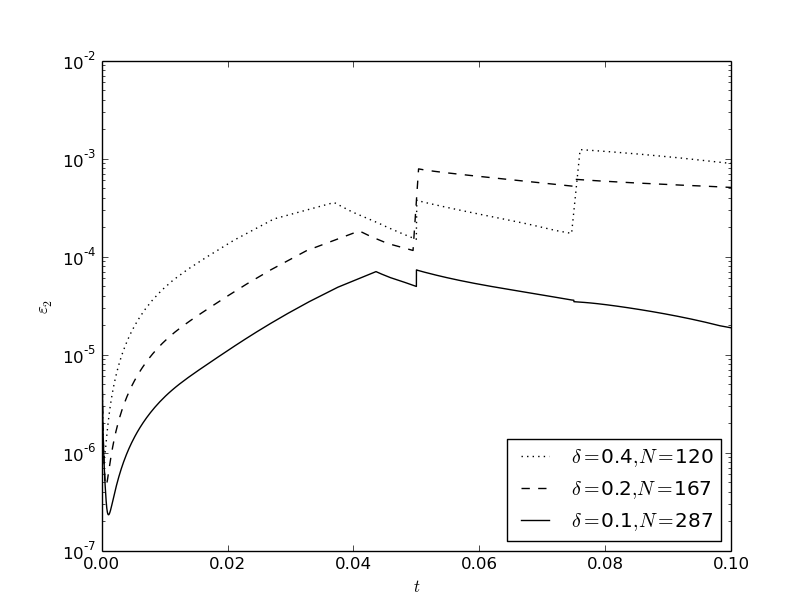
\includegraphics[width=0.8\linewidth] {ts_model/16.png}\\
	Error on irregular grid.
\end{center}
\end{frame}


\begin{frame}{Crank-Nicolson scheme}
\begin{center}
   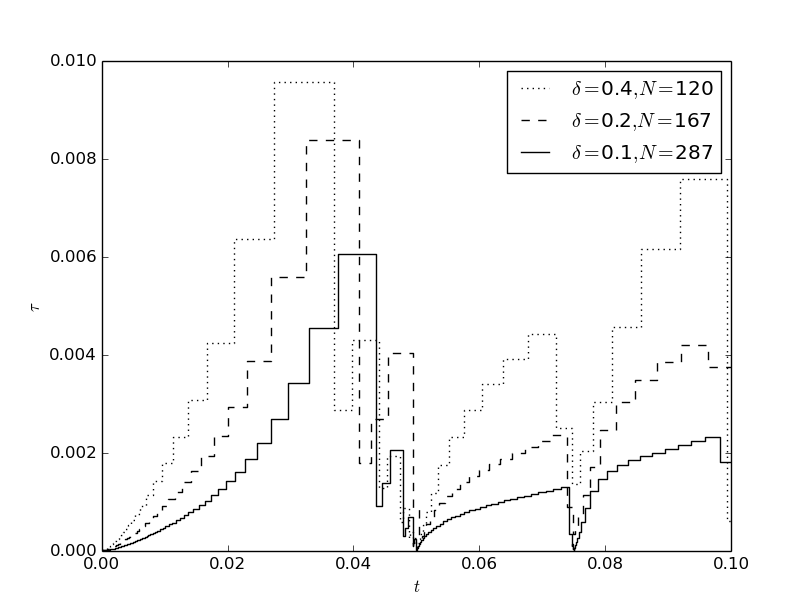
\includegraphics[width=0.8\linewidth] {ts_model/15.png}\\
	Time steps.
\end{center}
\end{frame}

\section*{Conclusion}
\begin{frame}{Conclusion}
\begin{itemize}
\item
An algorithm of time step selection for numerical solution of boundary problem for parabolic equations has been developed.
\vspace{2mm}

\item
The solution is obtained using guaranteed stable implicit schemes, and the step choice is performed with the use of the solution obtained by an explicit scheme.
\vspace{2mm}

\item
Calculation results obtained for a modal problem demonstrate reliability of the proposed algorithm for time step choice.
\end{itemize}

\vfill
\visible<2>{
\begin{center}
Thank you for your attention!
\end{center}
}

\end{frame}

\end{document}
